% В этом документе преамбула

%%% Работа с русским языком
\usepackage{cmap}					% поиск в PDF
\usepackage{mathtext} 				% русские буквы в формулах
\usepackage[T2A]{fontenc}			% кодировка
\usepackage[utf8]{inputenc}			% кодировка исходного текста
\usepackage[english,russian]{babel}	% локализация и переносы
\usepackage{indentfirst}			% чтобы первый абзац в разделе отбивался красной строкой
\frenchspacing						% тонкая настройка пробелов

%%% Приведение начертания букв и знаков к русской типографской традиции
\renewcommand{\epsilon}{\ensuremath{\varepsilon}}
\renewcommand{\phi}{\ensuremath{\varphi}}			% буквы "эпсилон"
\renewcommand{\kappa}{\ensuremath{\varkappa}}		% буквы "каппа"
\renewcommand{\le}{\ensuremath{\leqslant}}			% знак меньше или равно
\renewcommand{\leq}{\ensuremath{\leqslant}}			% знак меньше или равно
\renewcommand{\ge}{\ensuremath{\geqslant}}			% знак больше или равно
\renewcommand{\geq}{\ensuremath{\geqslant}}			% знак больше или равно
\renewcommand{\emptyset}{\varnothing}				% знак пустого множества

%%% Дополнительная работа с математикой
\usepackage{amsmath,amsfonts,amssymb,amsthm,mathtools} % AMS
\usepackage{icomma} % "Умная" запятая: $0,2$ --- число, $0, 2$ --- перечисление

%% Номера формул
\mathtoolsset{showonlyrefs=true} % Показывать номера только у тех формул, на которые есть \eqref{} в тексте.

%% Свои команды

% операции, не определённые (или имеющие иные обохначения) в мат. пакетах
\DeclareMathOperator{\sgn}{\mathop{sgn}}				% ф-ия sgn
\renewcommand{\tg}{\mathop{\mathrm{tg}}\nolimits}		% обозначение тангенса

%% Перенос знаков в формулах (по Львовскому)
\newcommand*{\hm}[1]{#1\nobreak\discretionary{}
{\hbox{$\mathsurround=0pt #1$}}{}}

%%% Работа с картинками
\usepackage{graphicx}  % Для вставки рисунков
\graphicspath{{images/}{images2/}}  % папки с картинками
\setlength\fboxsep{3pt} % Отступ рамки \fbox{} от рисунка
\setlength\fboxrule{1pt} % Толщина линий рамки \fbox{}
\usepackage{wrapfig} % Обтекание рисунков текстом

%%% Работа с таблицами
\usepackage{array,tabularx,tabulary,booktabs} % Дополнительная работа с таблицами
\usepackage{longtable}  % Длинные таблицы
\usepackage{multirow} % Слияние строк в таблице

%%% Теоремы
\theoremstyle{plain} % Это стиль по умолчанию, его можно не переопределять.
\newtheorem{theorem}{Теорема}[section]
\newtheorem{lemma}{Лемма}[section]
\newtheorem{definition}[theorem]{Определение}
\newtheorem{property}{Свойство}
 
\theoremstyle{definition} % "Определение"
\newtheorem{corollary}{Следствие}[theorem]
\newtheorem{exmp}{Пример}[section]
 
\theoremstyle{remark} % "Примечание"
\newtheorem*{nonum}{Решение}
\newtheorem*{evidence}{Доказательство}
\newtheorem*{remark}{Примечание}

%%% Программирование
\usepackage{etoolbox} % логические операторы

%%% Страница
\usepackage{extsizes} % Возможность сделать 14-й шрифт
\usepackage{geometry} % Простой способ задавать поля
	\geometry{top=25mm}
	\geometry{bottom=35mm}
	\geometry{left=35mm}
	\geometry{right=20mm}

%\usepackage{fancyhdr} % Колонтитулы
% 	\pagestyle{fancy}
 	%\renewcommand{\headrulewidth}{0pt}  % Толщина линейки, отчеркивающей верхний колонтитул
% 	\lfoot{Нижний левый}
% 	\rfoot{Нижний правый}
% 	\rhead{Верхний правый}
% 	\chead{Верхний в центре}
% 	\lhead{Верхний левый}
%	\cfoot{Нижний в центре} % По умолчанию здесь номер страницы

\usepackage{setspace} % Интерлиньяж (межстрочные интервалы)
%\onehalfspacing % Интерлиньяж 1.5
%\doublespacing % Интерлиньяж 2
%\singlespacing % Интерлиньяж 1

\usepackage{lastpage} % Узнать, сколько всего страниц в документе.

\usepackage{soulutf8} % Модификаторы начертания

\usepackage{hyperref}
\usepackage[usenames,dvipsnames,svgnames,table,rgb]{xcolor}
\hypersetup{				% Гиперссылки
    unicode=true,           % русские буквы в раздела PDF
    pdftitle={Заголовок},   % Заголовок
    pdfauthor={Автор},      % Автор
    pdfsubject={Тема},      % Тема
    pdfcreator={Создатель}, % Создатель
    pdfproducer={Производитель}, % Производитель
    pdfkeywords={keyword1} {key2} {key3}, % Ключевые слова
    colorlinks=true,       	% false: ссылки в рамках; true: цветные ссылки
    linkcolor=MidnightBlue,          % внутренние ссылки
    citecolor=black,        % на библиографию
    filecolor=magenta,      % на файлы
    urlcolor=blue           % на URL
}

\usepackage{csquotes} % Еще инструменты для ссылок

%\usepackage[style=authoryear,maxcitenames=2,backend=biber,sorting=nty]{biblatex}

\usepackage{multicol} % Несколько колонок

%%% Работа с графикой
\usepackage{tikz}
\usetikzlibrary{calc}
\usepackage{tkz-euclide}
\usetikzlibrary{arrows}
\usepackage{pgfplots}
\usepackage{pgfplotstable}

%%% Настройка подписей к плавающим объектам
\usepackage{floatrow}	% размещение
\usepackage{caption}	% начертание
\captionsetup[figure]{labelfont=bf,textfont=it,font=footnotesize}	% нумерация и надпись курсивом
% для подфигур: заголовок подписи полужирный, текст заголовка обычный
% выравнивание является неровным (т.е. выровненным по левому краю)
% singlelinecheck = off означает, что настройка выравнивания используется, даже если заголовок имеет длину только одну строку.
% если singlelinecheck = on, то заголовок всегда центрируется, когда заголовок состоит только из одной строки.
\captionsetup[subfigure]{labelfont=bf,textfont=normalfont,singlelinecheck=off,justification=raggedright}

%%% Stuff для графиков и рисунков



\title{Теория вероятностей и мат. статистика \\ ИДЗ3}
\date{04.05.2020}
\author{Почаев Никита Алексеевич, гр. 8381 \\ \href{mailto:pochaev.nik@gmail.com}{pochaev.nik@gmail.com} \\ Преподаватель: Малов Сергей Васильевич}

\begin{document}
	
\renewcommand{\figurename}{Рисунок}

\maketitle

\begin{figure}[H]
	\center{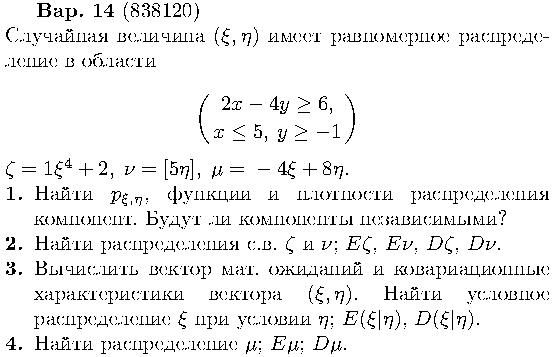
\includegraphics[scale=1]{./media/Задание.pdf}}
\end{figure}

Изобразим данную по условию область распределения случайной величины $(\xi, \eta)$ графически:
\begin{figure}[H]
	\center{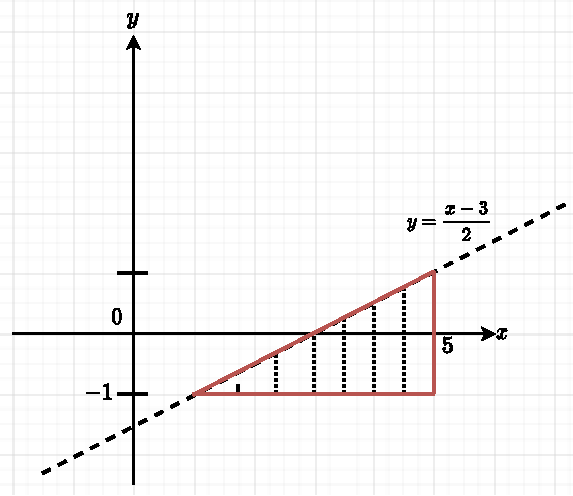
\includegraphics[scale=0.9]{./media/1_1.pdf}}
\end{figure}
Обозначим заштрихованную область распределения за $T$(riangle).

\begin{enumerate}
	\item Плотности распределения вероятностей системы $(\xi, \eta)$ равна:
	\[
		p_{\xi, \eta} =
		\begin{cases}
			C, x \in T \\
			0 - \text{ в остальных случаях}
		\end{cases}
		\text{, где } C - const
	\]
	
	Найдём константу $C$ из условия нормировки (интегрируем по области):
	\[
		\iint_{T} p_{\xi, \eta} (x, y) dxdy = \iint_{T} c dxdy = c \iint_{T} dxdy = c \cdot \left( \frac{4 \cdot 2}{2} \right) = 1 \Rightarrow c = \frac{1}{4}
	\]
	\begin{remark}
		\[ \iint_{T} p_{\xi, \eta} (x, y) dxdy \eq \int_{-\infty}^{\infty}\int_{-\infty}^{\infty} p_{\xi, \eta} (x, y) dxdy \]
	\end{remark}
	Таким образом,
	\[
		p_{\xi, \eta} (x, y) =
		\begin{cases}
			\frac{1}{4}, x \in T \\
			0 - \text{ в остальных случаях}
		\end{cases}
	\]
	
	\[
		p_{\xi} (x) =
		\begin{cases}
			\int\limits_{-1}^{\frac{1}{2}(x-3)} \frac{1}{4} dy = \frac{x-1}{8}, x \in [1, 5] \\
			0 - \text{ в остальных случаях}
		\end{cases}
		~~~~~~~~~
		F_{\xi} (x) =
		\begin{cases}
			0, &x \le 1 \\
			\int\limits_{1}^{x} \left(\frac{t-1}{8}\right) dt = \frac{1}{16} (x-1)^2, &x \in (1, 5] \\
			1, &x > 5
		\end{cases}
	\]
	
	\[
		p_{\eta} (y) =
		\begin{cases}
			\int\limits_{2y+3}^{5} \frac{1}{4} dx = \frac{1-y}{2}, y \in [-1, 1] \\
			0 - \text{ в остальных случаях}
		\end{cases}
		~~~~~~~~~
		F_{\eta} (y) =
		\begin{cases}
			0, &y \le -1 \\
			\frac{1}{2}\int\limits_{-1}^{y} (1-t) dt = \frac{1}{4} (-y^2+2y+3), &y \in (-1, 1] \\
			1, &y > 1
		\end{cases}
	\]
	Графики функций распределения представлены ниже:
	\begin{figure}[H]
		\center{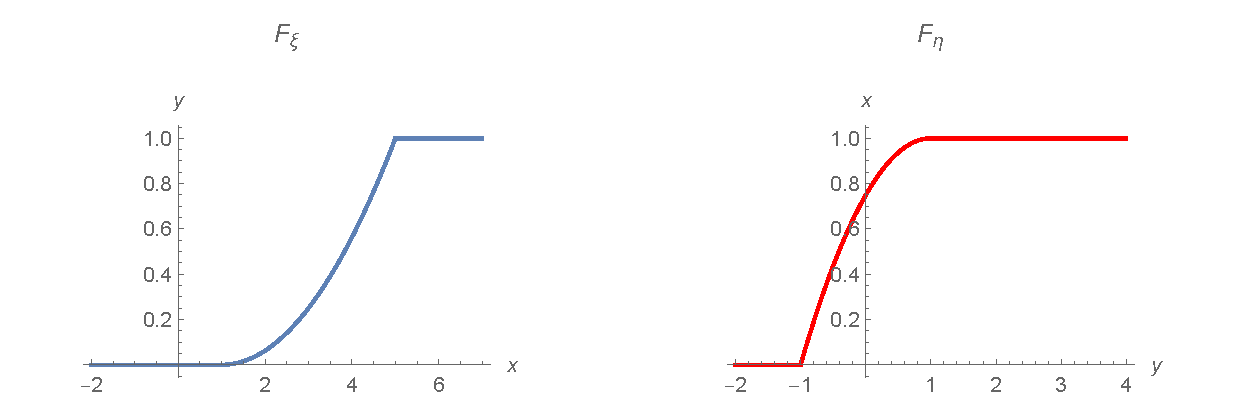
\includegraphics[scale=0.9]{./media/1_3.pdf}}
	\end{figure}
	
	Правильность вычисления плотностей и функций распределения частично доказывается выполнением свойств этих объектов. Для плотности: $p_{\xi} \ge 0, \int\limits_{-\infty}^{\infty} p_{\xi} (x) dx = 1$. Для функции распределения: $1 \le F_{\xi} (x) \le 5$ - неубывающая (данный факт также отражён на рис. ниже). Также можно показать, что $p_{\xi} = F_{\xi}'(x)$ или $F_{\xi} = \int\limits_{-\infty}^{x} p_{\xi} (x) dx$.
	\begin{figure}[H]
		\center{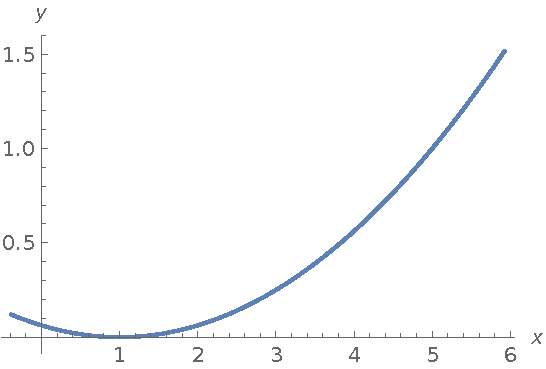
\includegraphics[scale=0.6]{./media/1_2.pdf}}
	\end{figure}
	
	Проверим независимость компонент. При $x=3, y$ может принимать единственное значение. 
	Пусть $x = 2, y = -0.5$, тогда
	\[ p_{\xi} (4) = \frac{2-1}{8} = \frac{1}{8} ~~~~~~~~~ p_{\eta} (-0.5) = \frac{1+0.5}{2} = \frac{3}{4} \]
	Плотность $p_{\xi, \eta} (x,y)$ нулевая при $2x - 4y \ge 6$, в данном случае $4 + 2 \ge 6$ - верно $\Rightarrow$
	\[ 0 = p_{\xi, \eta}(2, -0.5) \ne p_{\xi} (2) \cdot p_{\eta} (-0.5) = \frac{3}{32} \]
	Таким образом, очевидно, что величины зависимы.
	
	\item \[ \supp (\xi) = [1, 5], \supp (\zeta) = [3, 627] \]
	\[ F_{\zeta} (x) = P(\zeta < x) = P(\xi^4 + 2 < x) = P(\xi^4 < x - 2) = P(\underbrace{-\sqrt[4]{x-2} < \xi < \sqrt[4]{x-2}}_{\text{т.к. } \supp (\xi) > 0 \Rightarrow \text{ исп. верх. гран.}}) = \]
	\[ = P(\xi < \sqrt[4]{x-2}) = F_{\xi} (\sqrt[4]{x-2}) = \frac{1}{16} (\sqrt[4]{x-2} - 1)^2 \]
	
	Посчитаем через интегрирования, чтобы произвести проверку корректности вычислений:
	\[ F_{\zeta} (x) = P(\xi < \sqrt[4]{x-2}) = \int_{1}^{\sqrt[4]{x-2}} dx \int_{-1}^{\frac{x-3}{2}} \frac{1}{4} dy = \int_{1}^{\sqrt[4]{x-2}} \frac{x-1}{8} dx = \frac{1}{16} (\sqrt[4]{x-2} - 1)^2 \]
	Таким образом получили, что функция распределения с.в. $\zeta$ найдена верна.
	
	Итак, функция распределения:
	\[
	F_{\zeta} (x) =
	\begin{cases}
		0, &x \le 3 \\
		\frac{1}{16} (\sqrt[4]{x-2} - 1)^2, &x \in [3, 627] \\
		1, &x > 627
	\end{cases}
	\]
	График полученной функции представлен далее:
	\begin{figure}[H]
		\center{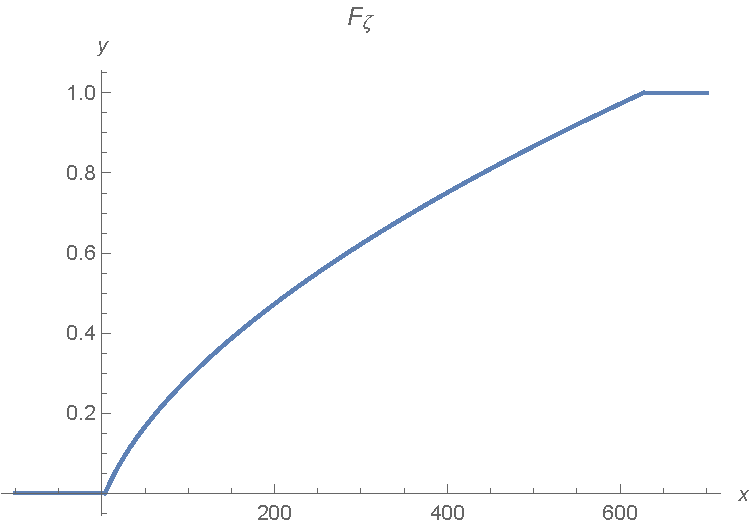
\includegraphics[scale=0.8]{./media/2_1.pdf}}
	\end{figure}
	Плотность распределения в свою очередь:
	\[
	p_{\zeta} (x) =
	\begin{cases}
		\frac{\sqrt[4]{x-2}-1}{32(x-2)^{\frac{3}{4}}}, x \in [3, 627] \\
		0 - \text{ в остальных случаях}
	\end{cases}
	\]
	Найдём мат. ожидание и дисперсию:
	\[ E\zeta = \int_{-\infty}^{\infty} x \cdot p_{\zeta} (x) dx = \int_{3}^{627} x \left(\frac{\sqrt[4]{x-2}-1}{32(x-2)^{\frac{3}{4}}}\right) dx = \]
	\[ = \frac{1}{32} \int_{3}^{627} \left( \frac{x}{\sqrt{x-2}} \right) dx - \frac{1}{32} \int_{3}^{627} \frac{x}{(x-2)^{\frac{3}{4}}} dx = \underset{\text{стандартные замены}}{\dots} = \frac{1247}{5} = 249.4 \]
	\[ E\zeta^2 = \int_{3}^{627} x^2 \left(\frac{\sqrt[4]{x-2}-1}{32(x-2)^{\frac{3}{4}}}\right) dx = \frac{4317173}{45} \approx 95937.178 \]
	\[ D\zeta = E\zeta^2 - (E\zeta)^2 = \frac{4317173}{45} - \left( \frac{1247}{5} \right)^2 = \frac{7590784}{225} \approx 33736.81 \bar{7} \]
	
	$\nu = [5 \eta]$ означает, что мы берём только значения $\in \mathbb{Z}$, а с.в $\nu$ - дискретная, т.е.
	\[ \supp(\eta) = [-1, 1], \supp (\nu) = \{-5,-4,-3,\dots,3,4,5\} \]
	\[ P(\nu = a) = P\left( \eta \in \left[ \frac{a}{5}; \frac{a}{5} + \frac{1}{5} \right] \right) = F\left(\frac{a}{5} + \frac{1}{5}\right) - F\left(\frac{a}{5}\right) = \]
	\[ = \frac{1}{4} \left( - \left( \frac{a+1}{5} \right)^2 + 2 \frac{a+1}{5} + 3 - \left( - \left(\frac{a}{5}\right)^2 + 2 \frac{a}{5} + 3 \right) \right) = \]
	\[ = \frac{1}{100} (9 - 2a) \]
	\[ \sum_{a=-5}^{4} \frac{1}{100} (9 - 2a) = 1 - \text{ ПГС}; ~~~~~~~~~ P(\nu = 5) = 0 \]
	Итак, функция распределения:
	\[
	F_{\nu} (t) = P(\nu < t) =
	\begin{cases}
		0, &t \le -5 \\
		\sum\limits_{a=-5}^{a < t} \frac{1}{100} (9 - 2a), &t \in (-5,5] \\
		1, &t > 5
	\end{cases}
	\]
	Найдём мат. ожидание и дисперсию:
	\[ E\nu = \sum_{t=-5}^{4} t \cdot \frac{1}{100} (9 - 2t) = -\frac{43}{20}; ~~~~~~ E\nu^2 = \sum_{t=-5}^{4} t^2 \cdot \frac{1}{100} (9 - 2t) = \frac{203}{20} \]
	\[ D\nu = E\nu^2 - (E\nu)^2 = \frac{203}{20} - \left( -\frac{43}{20} \right)^2 = \frac{2211}{400} = 5.5275 \]
	
	\item
	\[ E\xi = \int_{-\infty}^{\infty} x \cdot p_{\xi} (x) dx = \int_{1}^{5} x \left( \frac{x-1}{8} \right) dx = \frac{11}{3}; ~~~~~~ E\xi^2 = \int_{1}^{5} x^2 \left( \frac{x-1}{8} \right) dx = \frac{43}{3} \]
	\[ E\eta = \int_{-\infty}^{\infty} y \cdot p_{\eta} (y) dy = \int_{-1}^{1} y \left( \frac{1-y}{2} \right) dy = -\frac{1}{3}; ~~~~~~ E\eta^2 = \int_{-1}^{1} y^2 \left( \frac{1-y}{2} \right) dy = \frac{1}{3} \]
	\[ D\xi = E\xi^2 - (E\xi)^2 = \frac{43}{3} - \left(\frac{11}{3}\right)^2 = \frac{8}{9}; ~~~~~~ D\eta = E\eta^2 - (E\eta)^2 = \frac{1}{3} - \left(- \frac{1}{3}\right)^2 = \frac{2}{9} \]
	Вектор мат. ожидания: $E = \begin{pmatrix} \xi \\ \eta \end{pmatrix} = \frac{1}{3} \begin{pmatrix} 11 \\ -1 \end{pmatrix}$
	\[ E\xi\eta = \int_{\mathbb{R}^2} xy \cdot p_{\xi, \eta} (x,y) dxdy = \int_{1}^{5} dx \int_{-1}^{\frac{x-3}{2}} xy \cdot \frac{1}{4} dy = \int_{1}^{5} \frac{1}{32} x (x^2-6x+5) dx = -1 \]
	\begin{center}
		\fbox{%
			\parbox[t][6.5cm]{13cm}{%
				Пусть $\eta, \xi$ - две случайные величины, определённые на одном и том же вероятностном пространстве. Тогда ковариацией случайных величин (\textit{англ.} covariance) $\eta$ и $\xi$ называется выражение следующего вида:
				\[ \cov (\eta, \xi) = E((\eta - E\eta) \cdot (\xi - E\xi)) \]
				В силу линейности математического ожидания, ковариация может быть записана как:
				\[ \cov (\eta, \xi) = E (\xi \cdot \eta - \eta \cdot E\xi + E\xi \cdot E\eta - \xi \cdot E\eta) = \]
				\[ = E(\xi \cdot \eta) - E\xi \cdot E\eta - E\xi \cdot E\eta + E\xi \cdot E\eta = \]
				\[ = E(\xi \cdot \eta) - E\xi \cdot E\eta \]
		}}\qquad
	\end{center}
	\[ \cov (\xi, \eta) = -1 + \frac{11}{3} \cdot \frac{1}{3} = \frac{2}{9} \]
	Коэффициент корреляции:
	\[ r(\xi, \eta) = \frac{\cov (\xi, \eta)}{\sqrt{D\xi \cdot D\eta}} = \frac{\frac{2}{9}}{\sqrt{\frac{8}{9} \cdot \frac{2}{9}}} = \frac{1}{2} \]
	Матрица корреляции:
	\[ \corr \begin{pmatrix} \xi \\ \eta \end{pmatrix} = \begin{pmatrix} 1 & \frac{1}{2} \\ \frac{1}{2} & 1 \end{pmatrix} \]
	\begin{center}
		\fbox{%
			\parbox[t][3.5cm]{13cm}{%
				Матрица ковариаций (\textit{англ.} covariance matrix) — это матрица, элементы которой являются попарными ковариациями элементов одного или двух случайных векторов. Ковариационная матрица случайного вектора — квадратная симметрическая неотрицательно определенная матрица, на диагонали которой располагаются дисперсии компонент вектора, а внедиагональные элементы — ковариации между компонентами.
		}}\qquad
	\end{center}
	Матрица ковариации:
	\[ \var \begin{pmatrix} \xi \\ \eta \end{pmatrix} = \begin{pmatrix} D\xi & \cov (\xi, \eta) \\ \cov (\xi, \eta) & D\eta \end{pmatrix} = \begin{pmatrix} \frac{8}{9} & \frac{2}{9} \\ \frac{2}{9} & \frac{2}{9} \end{pmatrix} \]
	Условное распределение $\xi$ при условии $\eta$:
	\[
	p_{\xi|\eta = y_0} (x) = \frac{p_{\xi, \eta}  (x,y)}{p_{\eta} (y)} =
	\begin{cases}
		\frac{1}{2(1-y_0)}, x \le 5, y \ge -1, 2x - 4y \ge 6 \\
		0 - \text{ в остальных случаях}
	\end{cases}
	\]
	\begin{center}
		\fbox{%
			\parbox[t][3cm]{8cm}{%
				\[ f_{\xi | \eta} (x | y_0) \ge 0 \text{ почти всюду на } \mathbb{R}^{m+n} \]
				\[ \int_{\mathbb{R}^m} f_{\xi | \eta} (x | y_0) dx = 1, \forall y_0 \in \mathbb{R}^n \]
		}}\qquad
	\end{center}
	Проверим корректность вычислений, зафиксировав $y=0 \Rightarrow x = 3$: $\int\limits_{3}^{5} \dfrac{1}{2(1-0)}dx = 1$.
	\[
	p_{\xi | \eta} (x) =
	\begin{cases}
		\frac{1}{2(1-\eta)}, \text{ при } x \le 5, 2x - 4 \eta \ge 6 \\
		0 - \text{ в остальых случаях}
	\end{cases}
	\]
	Условное мат. ожидание:
	\[ E(\xi | \eta = y_0) = \int_{1}^{5} x \cdot p_{\xi | \eta = y_0} (x) dx = \int_{1}^{5} \frac{x}{2(1-y_0)} dx = -\frac{6}{y-1} \Rightarrow E(\xi|\eta) = \frac{-6}{\eta-1} \]
	\[ E(\xi^2 | \eta = y_0) = \int_{1}^{5} x^2 \cdot p_{\xi | \eta = y_0} (x) dx = \int_{1}^{5} \frac{x^2}{2(1-y_0)} dx = \frac{62}{3-3y_0} \]
	\[ D(\xi | \eta = y_0) = \frac{62}{3-3y_0} - \left( -\frac{6}{y_0-1} \right)^2 = -\frac{2(31y_0 + 23)}{3(y_0-1)^2} \Rightarrow D(\xi | \eta) = -\frac{2(31\eta + 23)}{3(\eta-1)^2} \]
	
	\item
	\[
	F_{\mu} (z) = P(-4\xi + 8 \eta < z) =
	\begin{cases}
		0, &z \le -28 \\
		*, &z \in (-28, -12] \\
		1, &z > -12
	\end{cases}, \supp (\mu) = [-28, -12]
	\]
	\begin{figure}[H]
		\center{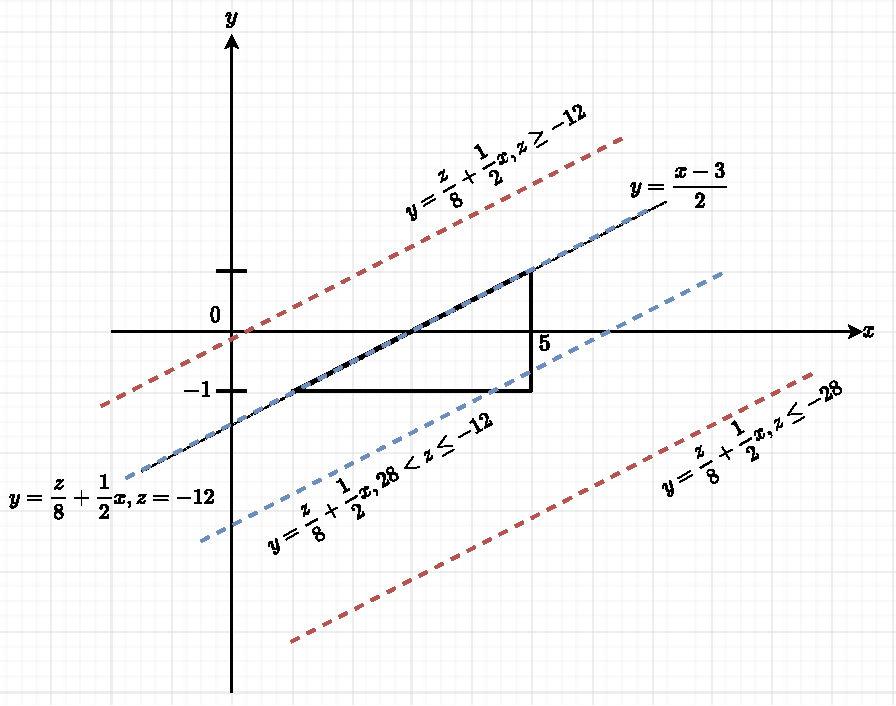
\includegraphics[scale=0.9]{./media/4_1.pdf}}
	\end{figure}
	При $z \in (-28, -12]: -4x + 8y = z, y = -1.5 \Rightarrow x = -\left(\dfrac{z}{4}+2\right)$.
	\[ * = F_{\mu}(z) = \int_{-\left(\frac{z}{4}+2\right)}^{5} dx \int_{-1}^{\frac{z}{8} + \frac{1}{2}x} \frac{1}{4} dy = \int_{-\left(\frac{z}{4}+2\right)}^{5} \frac{1}{32} (4x + z + 8) dx = \frac{1}{256} (z + 28)^2 \]
	Итак, функция распределения:
	\[
	F_{\mu} (z) = P(-4\xi + 8 \eta < z) =
	\begin{cases}
		0, &z \le -28 \\
		\frac{1}{256} (z + 28)^2, &z \in (-28, -12] \\
		1, &z > -12
	\end{cases}
	\]
	График функции приведён ниже:
	\begin{figure}[H]
		\center{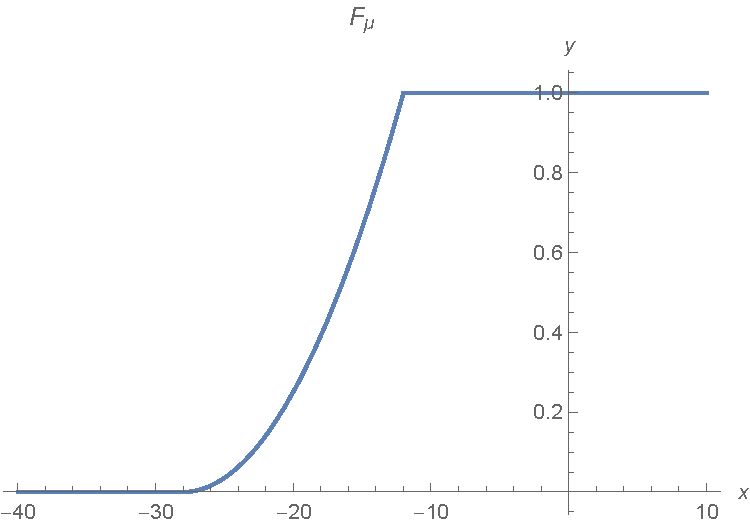
\includegraphics[scale=0.9]{./media/4_2.pdf}}
	\end{figure}
	\[
	p_{\nu} (z) =
	\begin{cases}
		\dfrac{z + 28}{128}, z \in [-28,-12] \\
		0 - \text{ в остальных случаях}
	\end{cases}
	\]
	\[ E\mu \int_{-28}^{-12} z \cdot \frac{z + 28}{128} dx = -\frac{52}{3} \approx -17.333; ~~~~~~~~~ E\mu^2 \int_{-28}^{-12} z^2 \cdot \frac{z + 28}{128} dx = \frac{944}{3} \approx 314.667 \]
	\[ D\mu^2 = E\mu^2 - (E\mu)^2 = \frac{944}{3} - \left( -\frac{52}{3} \right)^2 = \frac{128}{9} \approx 14.\bar{2} \]
	
\end{enumerate}

\end{document} 